Lock-in Amplifiers (LIAs) are amplifiers that extract the amplitude and phase of a signal with a known frequency from a noisy environment, as shown in \autoref{fig:LIA_principle}. They act as narrowband filter to precisely measure the amplitude of a signal hidden by noise \cite{Carminati2017,horowitz1989art}. \par 

\begin{figure}[ht]
    \centering
    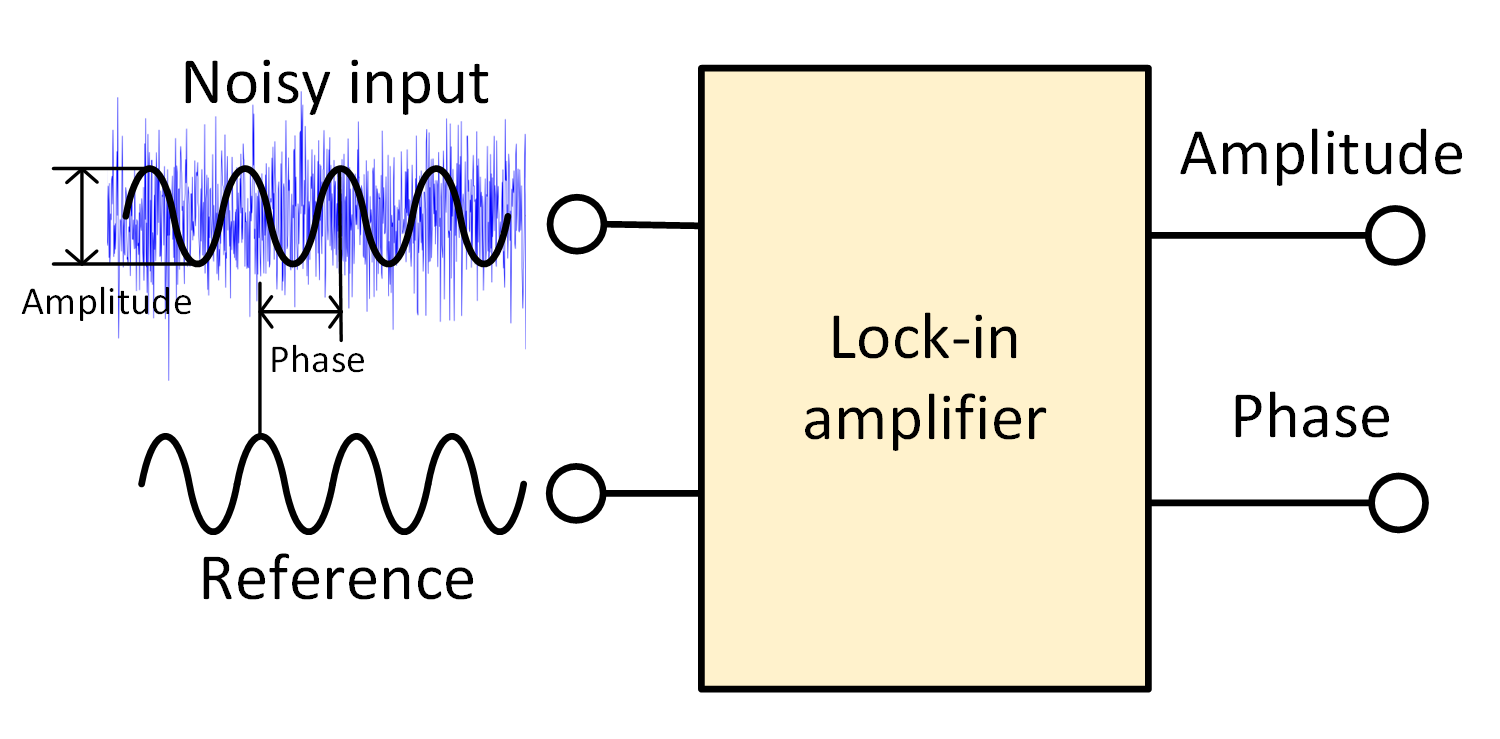
\includegraphics[width=0.7\textwidth]{LIA_principle}
    \caption{Basic principles of a LIA. The amplitude and phase components can be retrieved from a noisy environment.}
    \label{fig:LIA_principle}
\end{figure}
LIA work by transforming the desired AC signal into a DC signal with an amplitude proportional to the output of the measured signal. Some of these amplifiers use analog frequency mixers and other non-linear schemes to obtain the DC amplitude and then use low-pass filter with analog RC filters \cite{horowitz1989art} to isolate the DC signal \cite{Carminati2017}. The frequency-mixing can be achieved by multiplying the input waveform to a reference signal with the same frequency as the input. Mathematically, multiplying two signals together sends the fundamental of that signal to a DC value, as described in \autoref{fig:Mixing} and \autoref{eq:Mixing} :
\begin{equation}
\label{eq:Mixing}
   U_{mix} = U_{in}(f_1) \times U_{ref}(f_2) = \lvert U_{ref} \rvert \lvert U_{in} \rvert \frac{1}{2} (cos(f_1 - f_2) - cos(f_1 + f_2))
\end{equation}
\begin{figure}[ht]
\centering
\begin{subfigure}{0.35\textwidth}
\centering
    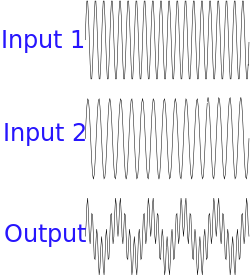
\includegraphics[width=0.8\linewidth]{MixingTime}
    \caption{In time.}
\end{subfigure}
\begin{subfigure}{0.64\textwidth}
\centering
    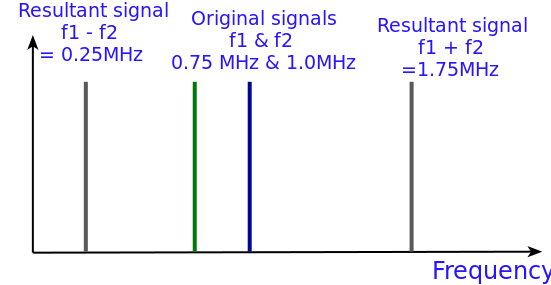
\includegraphics[width=0.9\linewidth]{MixingFreq}
    \caption{In frequency.}
\end{subfigure}
\caption{Mixing two sinewaves of frequency $f_1$ and $f_2$ result in two output signals at frequency $f_1-f_2$ and $f_1 + f_2$ \citep{poole_2020}.}
\label{fig:Mixing}
\end{figure}
For identical frequencies between the reference and input signals and after filtering the high frequency component, only a DC component remains \cite{Carminati2017}, which has an amplitude proportional to half the multiplication of the two signals amplitude: 
\begin{equation}
   \Re(U_{mix-LPF}) = \lvert U_{ref} \rvert \lvert U_{in} \rvert \frac{1}{2} cos(\phi)
\end{equation}
This system can be called a single-phase LIA since a unique in-phase signal has been used for mixing \cite{horowitz1989art}. The phase component $\phi$ in a single-phase LIA can create a significant error if some delay or parasitic capacitances are present in the system and the angle $\phi$ gets further away from 0°. By using a two-phase LIA in quadrature-mode, it is possible to remove the precision loss caused by the unknown phase parameter \cite{horowitz1989art}. Being in quadrature mode means that two reference signals are used, one called the in-phase component at a phase of 0°, and a quadrature component which is phase-shifted by 90°. This creates an in-phase real output $\Re(U_{mix-LPF})$ which depends on the cosine of the angle $\theta$ and a quadrature imaginary output $\Im(U_{mix-LPF})$ which depends on the sine. Using \autoref{eq:Magnitude} and \autoref{eq:Phase}, it is possible to deduce the actual magnitude and phase of the original signals: 
\begin{equation}
   \Im(U_{mix-LPF}) = \lvert U_{ref} \rvert \lvert U_{in} \rvert \frac{1}{2} sin(\phi)
\end{equation}
\begin{equation}
   \lvert U_{mix-LPF} \rvert = \sqrt{\Re(U_{mix-LPF})^2 + \Im(U_{mix-LPF})^2}
\end{equation}
\begin{equation}
   \phi = \atan(\frac{\Im(U_{mix-LPF})}{\Re(U_{mix-LPF})})
\end{equation}
The state-of-the-art LIA is digital since the signal multiplication can be done very efficiently and the phase difference between two signals can be measured precisely using zero crossing algorithms. The mixing scheme of LIA can be implemented efficiently inboard microprocessors or FPGA. However, they are only usable for low to middle frequencies since the signals must first be sampled by the processor’s ADC, which has a limited MCLK frequency \cite{horowitz1989art} This is why analog mixers are used in this project.